\documentclass{article}
\usepackage{amsmath}
\usepackage{amssymb}
\usepackage{graphicx}
\usepackage[margin=1in]{geometry}
\setlength{\parindent}{0in}
\setlength{\parskip}{0.05in}

\title{Lecture notes, ISTA 331 Curve Fitting Day 1}

\begin{document}
\maketitle

\textit{Summary: The goal today is to review and explore the idea of fitting a model by optimization. Part 1 is thinking of the mean as the solution to a model-fitting problem (where our model is just a number). Part 2 is simple linear regression (which should be review since you did the OLS lab already). Part 3 is introducing the ideas of curve fitting with more general functions, starting with using log transformations so that you can fit a power law with simple linear regression. If there is time, we can talk about trying to fit a sinusoid to some data. The students get a Jupyter notebook with some code (mostly the plots, since those take a lot of tweaking to refine) and some empty cells for definitions/notes.}

\textit{Bolded questions are questions that you can pose to the class (but don't try to get an answer from them for every question, as that would probably take too long.)}

\section*{Day 1}

\subsection*{Basic ideas}

\textbf{Why are we doing data science?} Basically, we want to predict the future.

\textbf{How do we do this?} We have some sample observations; choose a model for the target variable, and try to find the parameters of our model that fit the observations as well as possible.

\subsubsection*{Super simple example}

Sometimes this process is so simple you don't even think of it as ``model fitting.'' Say I'm planning a trip for 6 months from now. I want to know what the chance is it will rain at my destination, so that I can decide what to pack or where to go. What should I do?
\begin{itemize}
    \item Probably, I will go on Google and look up the average chance of rain in August wherever I'm going.
    \item I'm using a mean as a \textbf{predictive model}.
    \item My target variable is the chance of rain. Someone else collected the data and calculated the mean.
    \item If historically it rained 23\% of all August days, I predict the chance it will rain on any given day this August is 23\%.
\end{itemize}
How well does my model describe reality? Well, that depends:
\begin{itemize}
    \item If the historical \% of rain looks like
    \[
    [21\%, 23\%, 22\%, 25\%, 26\%, 23\%, \ldots]
    \]
    then my model is pretty good.
    \item If the historical \% of rain looks like
    \[
    [3\%, 6\%, 0\%, 86\%, 5\%, 0\%, 91\%, \ldots]
    \]
    then I might have the same mean but it's not a good prediction.
\end{itemize}

\textbf{What number can you calculate to describe the difference between those two?} Think back to intro stats. Answer: the standard deviation. What's the formula?
\[
    s = \sqrt{\frac{1}{N-1} \sum_{i=1}^N (y_i - \bar y)^2}
\]
AKA: root-mean-square error (RMSE), but usually not called this in the context of the mean. It measures variability around the mean. If the standard deviation is big, the mean is less likely to be an accurate prediction. Sometimes people use $\sigma$ for the above, but really $\sigma$ means the population std. dev., which is almost always unknown.

So the RMSE / standard deviation can be thought of as a measurement of how well a single point fits the data. This is called \textbf{goodness of fit.}

\textit{Draw a sketch version of this:}

\begin{center}
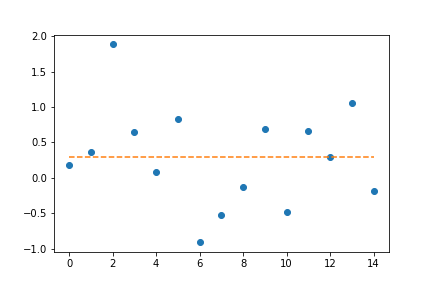
\includegraphics[width=3in]{meanplot.png}
\end{center}

\textit{Sketch a residual on the plot, or ask a student to come up and sketch one.} Notice that this difference between the observation and the mean line is measured by $y_i - \bar y$. So the RMSE / standard deviation is averaging the squares of these residuals (sort of).
Sometimes the residuals are called the errors, but this is slightly bad terminology: the ``error'' we are interested in is the error in future predictions. This residual is a prediction of that future error.

\textbf{Aside}: what is the $1$ in the formula called and what is it for? $N$ is the number of degrees of freedom (number of data points); we adjust by the number of parameters we are fitting (hence, $-1$ because our only parameter is the mean). The 1 is called \emph{delta degrees of freedom} (\texttt{ddof} in scipy calculations). This reduces bias in the estimate. The sample std. dev. $s$ is a biased estimate of $\sigma$ because it is calculated from differences between observations and the sample mean, not the population mean. The sample mean is naturally closer to the sample than the population mean, so the sample std. dev. is a little too small in general.

How is calculating the mean like fitting a model?
\begin{itemize}
    \item My ``model'' here is extra simple: it's just one number. The only prediction I ever make is that number.
    \item Once I decide to make this model, I just have to pick the number that fits the data best.
    \item What number fits the data best? The mean.
\end{itemize}

\textbf{Question: what does best mean?} If you write the formula above as a function of $\bar x$, like
\[
    s(\bar y) = \sqrt{\frac{1}{N-1} \sum_{i=1}^N (y_i - \bar y)^2}
\]
and you pretend you didn't know $\bar y$ stands for the mean, you could calculate this plugging in a bunch of different numbers for $\bar y$.

\textit{Activity: Go to the Jupyter notebook. There is a function to calculate this in there, called \texttt{rmse}. Have the students call this function to calculate it plugging in a few different values for y. Once they've tried a few values, have them pass it the mean of the data. Notice that it's smaller than any of the other values they got.}

The best-fitting model in this sense is the one that gives us the smallest RMSE calculated with respect to that point; turns out that's always the mean. (If you know Calculus I, you can prove this in a few lines.) So calculating the mean is getting the ``best fit point'' for a set of data, as measured by RMSE.

\textbf{Optimization:} finding the input that gives the maximum or minimum output of a function. Fitting a model almost always means finding some way to measure goodness of fit, then optimizing it. If you choose a different measurement to optimize, you get a different fit.

\textbf{Example:} What if we went with a seemingly simpler option? Measure the ``distance'' from our model to the data by averaging the absolute difference between each point and the model:
\[
    s_1(y^*) = \frac{1}{N - 1} \sum_{i = 1}^N |y_i - y^*|
\]
(I use the $*$ here to avoid using $\bar y$ because we all know that means the mean. But $y^*$ is just a model parameter here.) What would our model estimate be now? It's another number you're all familiar with from basic stats -- can you guess it? Answer: the median! (This isn't quite as easy to prove.)

Why is it more common to use the first one? Several reasons, but simpler math is a big one. The absolute value function has a sharp corner, and that makes it hard to minimize.

\subsubsection{Fitting curves}

Let's look at an example. This example has come from past 131 sections, so you may have seen it before; and you did OLS in the lab a couple of weeks ago, so this should be mostly review. We have some data on sea ice extent.

\textit{In the Jupyter notebook we calculate the annual mean, and then the overall mean. First two plots are line plot of sea ice extent over time; the second one has the overall mean plotted as a horizontal line. After the second one is }

\textbf{What's the problem with this model?} What does it predict for sea ice in 2030? 2050? 2100? Always the same value: 11.47 million $\mathrm{km}^2$. But there is an obvious trend over time in this data.

\textbf{Choose a model.} Simplest model: ice is a linear function of time:
\[
\hat y = ax + b = a(\mathrm{time}) + b
\]
Now we have to fit two parameters.

\textbf{How do we find the best fit line?} OLS. This is again a matter of optimizing a measure of goodness of fit.

\textbf{What is the analogue of the standard deviation for OLS?} Again it's RMSE:
\[
    RMSE = \sqrt{\frac{1}{N-2} \sum_{i=1}^N (y_i - \hat y)^2}
\]
Here $\hat y$ is the predicted value of $y$ at the same $x$-value as the observation $y_i$. Note $N - 2$: since we are fitting 2 parameters, delta degrees of freedom is 2.

\textbf{What are some other measures of goodness-of-fit we could minimize?}
\begin{itemize}
    \item Geometric distance between the points and the line. This would be like measuring the residual with the perpendicular distance to the line instead of the vertical distance. This would be harder to calculate and it would confound the relationship between $x$ and $y$ (because the residual wouldn't depend only on $y$-values at one value of $x$, but also on nearby values of $x$). So we don't do that.
    \item Mean absolute residual:
    \[
        \frac{1}{N - 1} \sum_{i = 1}^N |y_i - \hat y|
    \]
    People do this! It's called $L^1$ minimization and although it's somewhat harder to calculate, it produces better results in some contexts; there are applications in signal processing and medical imaging. But we'll stick with least squares.
\end{itemize}

Let's make a few predictions. \textit{(Have the students do this in the notebooks.)}

\textbf{What will be the mean extent of sea ice in 2030?}

\textbf{When will the mean extent be 0 -- that is, when should we expect no ice left?}
\textit{For this one, do the algebra at the board, but ask the students to calculate it numerically with some Python code.}

\textbf{Which of these predictions should we trust more?} The first. \textbf{Why?} The other extrapolates much farther into the future.

Why is this kind of extrapolation risky? Even if the fit is good now, the trend may change in the future.
\begin{itemize}
    \item For example, melting ice releases trapped carbon, accelerating warming. We could incorporate this into our model if we knew how. More complex models often use \emph{domain-specific knowledge}, i.e. expertise about the specific process being modeled. A climatologist might know what kind of function to add to the model to account for this effect, but we're not climatologists.
    \item More optimistically, reduced future emissions could slow warming. This would be very hard to predict because it's partly a social/political process, not just a physical one. So we might have to build a new model in 10 years.
\end{itemize}

Now let's compare the two models. By plotting both we can see that the residuals are much smaller when we use a linear model; this means the predictions more closely match the observations.

We can get a full summary of the model with \texttt{results.summary()}. There's a lot of information here, but some of the most important things are the 

\textit{After you get through the whole linear model for sea ice, there is some terminology:}

\textbf{Model:} We didn't actually define what we mean by a model, so now we'll say a model is one or more equations that describe some data or explain a relationship between variables.

\textbf{Sum of squared error, SSE:} The sum of the squared residuals:
\[
    \sum_{i=1}^N (y_i - \hat y)^2
\]

\textbf{Mean squared error, MSE:} The average of the squared residuals (adjusted by delta dof). 
\[
    \frac{1}{N - \mathrm{ddof}}\sum_{i=1}^N (y_i - \hat y)^2
\]

\textbf{Root mean squared error, RMSE:} Saw this above, the square root of MSE. Note that minimizing any of these three minimizes all of them, you can think of least squares as minimization of any of the above -- traditionally, it's SSE, but MSE or RMSE is usually a more useful measure because it's mostly independent of your sample size.
\[
    \sqrt{\frac{1}{N - \mathrm{ddof}}\sum_{i=1}^N (y_i - \hat y)^2}
\]

\textbf{What's another name for the process of fitting a line to the points?} Simple linear regression.

\textbf{Ordinary least squares:} the optimization process we did above, finding the best fit line by minimizing SSE, etc.

\textbf{Multiple linear regression:} Linear regression, but with more variables. For example, we could use some measure of ``storminess'' as a separate predictor of ice extent:
\[
    \widehat{\mathrm{extent}} = \mathrm{e_0} + m_1 \times \mathrm{Time} + m_2 \times \mathrm{Storminess}
\]
Can be fit by OLS in much the same way.

\textbf{Coefficient of Determination $R^2$}: Measures the amount of variation in $y$ that is accounted for by the model. In simple linear regression, the coefficient of determination is the square of the correlation coefficient $r$, but in other contexts it may not be. However, the notation $R^2$ is common even if it is not literally the square of a number called $R$.

\textbf{Polynomial regression:} Instead of fitting the data to a linear model, we fit to a polynomial function:
\[
    \hat y = a_0 + a_1 x + a_2 x^2 + \ldots + a_n x^n
\]
The highest power $n$ is called the \emph{degree} of the model. This is a hyperparameter (i.e. we have to choose it before fitting the model).

\subsubsection*{Fitting a nonlinear model with simple linear regression}

Now we'll ``cheat'' a bit and get a nonlinear model without any new regression methods.

We have data on planet's semi-major axis $r$ (the radius of the orbit along the long axis) and orbital period $T$ (how long it takes to orbit once.)
Plot it. \textbf{Are the two quantities related?} Yes, definitely. \textbf{Is the relationship linear?} No.

Here's a trick. Plot the same two quantities on a log scale. \textbf{What do you see?} (They should see points on a line.)

\textit{On the board:}
The idea is that we make a guess that a power function might fit (like we guessed a line might fit the sea ice). A power function looks like this:
\begin{align*}
T &= C r^p \\
\log y &= \log C + p * \log x
\end{align*}
After taking logs, the power model is a linear model. So we can fit a line and get a curve for free.

Fit the OLS model and take a look at the coefficients. What is the power $p$? (It should be very close to 1.5.)
Kepler's third law predicts 
\[
T^2 = \mathrm{const} \times r^3
\]
which is the same as the equation we got:
\[
\hat T = \mathrm{const} \times r^{1.5}
\]
So our curve fitting finds this physical law. (This is also why the curve fit is so good -- notice $R^2 \approx 1$. We're working with a physical law and the data has very little noise. Usually we won't get fits this good!)

\textit{If you have time at the end:}

Choosing a correct model often involves either domain-specific knowledge, standard tricks like log transforms, or enough mathematical knowledge to recognize a function from a plot.

Plot the data from \texttt{curvedat.csv}. What kind of mathematical function should fit this data? \texttt{Answer: a sin/cos}.

\textbf{How many parameters do we need for a sinusoid?} Three:
\[
    \hat y = A \sin(\omega(x + \phi))
\]

Can we eyeball the parameters for a good fit for this data? What do each of $A$, $\omega$, and $\phi$ represent?

\section*{Day 2}

\subsection*{Review}

\textbf{Last time:}
\begin{itemize}
    \item 
    \item 
    \item 
\end{itemize}

\subsection*{Statistical significance and $p$-values}

\textbf{What is a p-value?}

\textbf{How do you get a p-value?}

\textbf{}


\subsection*{Nonlinear least squares}




\end{document}